\section{Results}
\label{sec:results}

\subsection{Student versus prompted baselines}
\label{sec:main}

Table~\ref{tab:main} compares the student with schema-in-prompt (SIP) baselines: the same prompt---descriptions of the
functions, the three actions, the same data policy and three examples, about 2,150 tokens---given to the untrained
Qwen2.5-1.5B-Instruct and to the 72B teacher, each run once with greedy decoding.

\begin{table*}[t]
\centering\small
\setlength{\tabcolsep}{5pt}
\begin{tabular}{@{}lccccccc@{}}
\toprule
& \multicolumn{3}{c}{Clean test (230)} & Suppl. & Ambig-4 & Prompt & p50 \\
\cmidrule(lr){2-4}
System & Clear (74) & Amb. (39) & OOS (117) & (28) & (129) & tokens & latency \\
\midrule
Qwen2.5-1.5B, prompted (SIP) & 37.8 & 35.9 & 31.6 & 14.3 & 20.9 & 2,156 & 779\,ms \\
Qwen2.5-72B teacher, prompted (SIP) & \textbf{83.8} & 56.4 & \textbf{94.9} & 39.3 & 70.5 & 2,156 & 1,842\,ms \\
\midrule
Student v5, LoRA & 78.4 & 75.6 & 83.8 & 58.9 & 78.3 & 33 & \multirow{3}{*}{224\,ms$^{\dagger}$} \\
Student v6.1, LoRA & 78.4 & 75.6 & 77.4 & 58.9 & \textbf{79.1} & 33 & \\
Student v6.1 + threshold 0.85 & 75.0 & 74.4 & 82.1 & 58.9 & \textbf{79.1} & 33 & \\
\midrule
Deployed: v6.1 s42, 4-bit, $\tau$ 0.80 & 77.0 & 64.1 & 88.0 & 50.0 & 74.4 & 33 & 520\,ms$^{\ddagger}$ \\
\bottomrule
\end{tabular}
\caption{Accuracy (\%) on the frozen evaluation sets. Student rows are means of two seeds, unquantized; baselines are single
greedy runs; OOS = out-of-scope. Latency: A100 with vLLM, one query at a time ($^{\dagger}$measured for an earlier student
with the same prompt length); $^{\ddagger}$laptop CPU, llama.cpp. The v5 row comes from the same re-generation as v6.1 and differs by at most two items per group from the original v5
run in Table~\ref{tab:lora}. The deployed row is one seed after 4-bit quantization with the threshold
(\S\ref{sec:quant}).}
\label{tab:main}
\end{table*}

\paragraph{Training is necessary.} With the same 1.5B model, prompting reaches only 14--38\% on every group (21--28\% on the
newer short, two-turn, typo and Ambig-4 sets, Table~\ref{tab:v6}); the 1.5B prompted model over-triggers on 63\% of
out-of-scope requests and returns invalid JSON for 10 clean-test items. Fine-tuning with functional tokens roughly doubles to
quadruples every group while the prompt is 65 times shorter.

\paragraph{Against the 72B teacher.} Exact McNemar tests per seed (v6.1, unquantized, Appendix~\ref{app:seeds}) give:
\emph{clear commands} 81.1 and 75.7 vs.\ 83.8 ($p=0.77$, $0.15$): no detectable difference; \emph{long implicit requests}
(Ambig-4) 79.8 and 78.3 vs.\ 70.5 ($p=0.065$, $0.14$): higher but not significant; the small ambiguous group: significant for
one seed only (tie or slightly better); \emph{out-of-scope} 82.9 and 71.8 vs.\ 94.9 ($p\le0.001$ for both): the teacher is
clearly better. On the v6 sets (Table~\ref{tab:v6}; the prompted baselines were run on them later with the same prompt and
decoding) the picture is similar: \emph{short commands and paraphrases} 88.3 and 87.5 vs.\ 91.7 ($p=0.39$, $0.27$) and
\emph{typos} 60.6 and 66.3 vs.\ 69.2 ($p=0.093$, $0.66$) are ties, \emph{new arguments} favor the student (83.3 vs.\ 70.0,
$p=0.34$), but on \emph{two-turn follow-ups} the teacher is clearly better (81.7 vs.\ 66.7 and 58.3; $p=0.049$, $0.001$),
although it never saw a two-turn example and receives exactly the previous call that the student receives. Part of the 72B's errors on clear commands are label conventions it cannot know from descriptions (an AC
temperature without \code{state="on"}, ``weak lights'' $\rightarrow$ high beam). A 1.5B model can tie a 72B one on clear and
implicit requests here because the comparison is not symmetric: the student learned this task's conventions from 33k
examples of the teacher's \emph{filtered} outputs, whereas the teacher works zero-shot from a prompt; where general knowledge
or reasoning over context is needed---recognizing what the car cannot do, or how a follow-up modifies the previous
action---the larger model remains ahead.

\subsection{What the data rounds taught}
\label{sec:rounds}

\begin{figure*}[t]
\centering
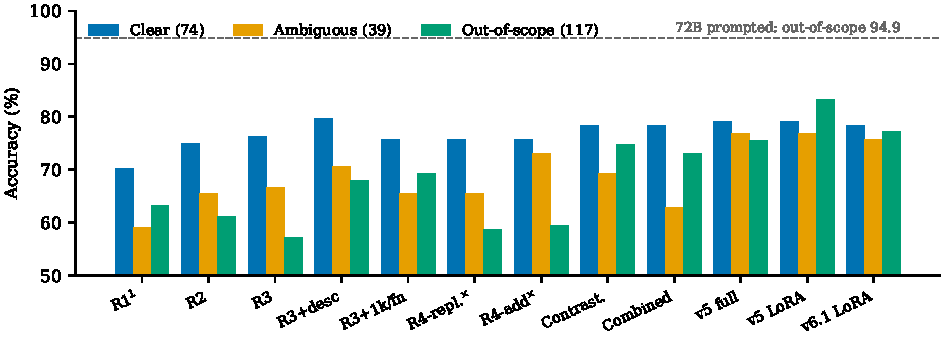
\includegraphics[width=\textwidth]{figures/rounds.pdf}
\caption{Clean-test accuracy across data configurations (means of two seeds; $^{1}$single seed; $^{\times}$rejected by
pre-registered criteria because they refused doable requests). The v6.1 row is from a later re-run of the same scorer.}
\label{fig:rounds}
\end{figure*}

Figure~\ref{fig:rounds} traces clean-test accuracy over the configurations we trained and Table~\ref{tab:ablation} gives the
side experiments on top of R3. Five findings shaped the final data.

\paragraph{Validation is not a test.} From R1 on, validation accuracy on clear commands was 97--99\%, while the clean test gave
65--80\%. Validation data come from the same teacher and prompts as training data, so they share its blind spots; only the
separately generated test sets revealed them.

\paragraph{Lexical lock-in.} In R1, 15 of 24 functions had one word covering $\ge95\%$ of their training sentences. All 267
window sentences said \textit{cửa sổ} (window) and none said \textit{kính} (glass), while every defrost sentence said
\textit{kính}; the model learned ``\textit{kính} $\Rightarrow$ defrost'' and turned \vi{Hạ kính ghế phụ}{lower the passenger
glass} into \code{set\_defrost(state="down")}. Asking the teacher to spread synonyms evenly (R2) fixed this: all nine
\textit{kính} window commands in the clean test now chose the window function, and window accuracy rose from 30\% to 80\%.

\paragraph{Shortcuts from sentence form.} R1 refusals were almost never imperative (2.1\%), so ``imperative $\Rightarrow$ call''
was 94.7\% accurate on the training data. Adding 1,667 imperative refusals in R2 broke this rule (60.4\%) but did not reduce
over-triggering (18.7\% $\rightarrow$ 17.8\%). In R4 we generated 1,651 refusals that first describe a situation and then ask
for something the car cannot do. Development-set refusals jumped from 8.5/20 to 20/20, but story-like \emph{doable} requests
were now refused (2--6 of 10, vs.\ 10/10 before): the model had learned ``story $\Rightarrow$ refuse''. Both R4 variants were
rejected by their pre-registered false-refusal criterion. Adding the same story frame on the call side (1,641 story-like calls,
the \emph{contrastive} configuration) removed the shortcut and gave the largest out-of-scope gain of the project
(57.2 $\rightarrow$ 74.8, with 10/10 doable requests kept). We now generate hard examples only in pairs across labels.

\paragraph{The same lesson for clarifications.} On a new 130-item ambiguous set (Ambig-3) with a pre-registered test, the
prompted 72B beat the contrastive student clearly (71.5 vs.\ 51.5 and 38.5; $p<0.001$ for both seeds). The student collapsed
on long, story-like complaints, mostly by refusing them. Training data explained why: among sentences longer than ten words
there were 3,254 refusals but only 102 clarifications. Round v5 added 1,696 story-like clarifications (a third contrastive
pair), judged by the jury and audited (90.4\%). On a fresh set, Ambig-4, v5 reached 74.4 and 72.1 vs.\ 51.2 and 45.0 for the
contrastive model ($p<10^{-4}$, both seeds) and became indistinguishable from the 72B (70.5; $p=0.51$, $0.87$); false
refusals on long complaints fell from 18 and 32 to 6 and 6, the 72B's level.

\paragraph{Octopus-style descriptions and data scale.} Appending function descriptions to targets raised clear commands by
3.4 points with almost no seed spread; using up to 1,000 samples per function (all of the pool) raised out-of-scope accuracy by
12 points. Combining both with the contrastive data brought no further gain: data scale and contrastive refusals fix the
same weakness, and the description effect was diluted (Table~\ref{tab:ablation}). We kept the smaller contrastive set
(17.6k vs.\ 30.0k examples) as the base for v5.

\begin{table}[t]
\centering\small
\setlength{\tabcolsep}{3pt}
\begin{tabular}{@{}lccccc@{}}
\toprule
Config. (vs.\ R3) & Clear & Amb. & OOS & Dev ref. & Dev do \\
\midrule
R3 & 76.3 & 66.7 & 57.2 & 8.5 & 10 \\
+ descriptions & \textbf{79.7} & 70.5 & 68.0 & 7.0 & 10 \\
+ 1,000 / function & 75.7 & 65.4 & 69.2 & 10.0 & 10 \\
R4 replace$^{\times}$ & 75.7 & 65.4 & 58.6 & 20.0 & 6 \\
R4 add$^{\times}$ & 75.7 & 73.1 & 59.4 & 20.0 & 2 \\
Contrastive & 78.4 & 69.2 & \textbf{74.8} & 17.5 & 10 \\
Combined & 78.3 & 62.8 & 73.0 & 16.5 & 10 \\
\bottomrule
\end{tabular}
\caption{Data experiments on top of R3 (full fine-tuning, means of two seeds). Dev ref.: refusals correct out of 20; Dev do:
doable story-like requests executed out of 10. Seed spreads are in Appendix~\ref{app:rounds}.}
\label{tab:ablation}
\end{table}

\subsection{LoRA versus full fine-tuning}
\label{sec:lora}

Octopus~v2 reports full fine-tuning slightly above LoRA (99.524\% vs.\ 99.048\%, which corresponds to one item if their test
has 210 queries). On the v5 data, with the same learning rate, seeds and selection rule, LoRA matches full fine-tuning on
clear commands and is better on out-of-scope requests (Table~\ref{tab:lora}). The out-of-scope advantage holds in all four
comparisons at equal epochs (two epochs $\times$ two seeds, +5 to +13 points); the advantage on Ambig-4 disappears at equal
epochs, so we attribute it to checkpoint choice. Full fine-tuning showed signs of overfitting (validation loss rising at
epoch 3, over-triggering growing with epochs). Lowering its learning rate to $2\times10^{-5}$ did not close the gap (76.1 on
out-of-scope; pre-registered verdict ``still behind'') and left the model under-trained on everything else. We therefore
deploy LoRA, but do not claim LoRA is better in general.

\begin{table}[t]
\centering\small
\setlength{\tabcolsep}{4pt}
\begin{tabular}{@{}lccc@{}}
\toprule
v5 data, mean of 2 seeds & Full $5\mathrm{e}{-5}$ & Full $2\mathrm{e}{-5}$ & LoRA \\
\midrule
Clear (74) & 79.1 & 71.6 & 79.1 \\
Ambiguous (39) & 76.9 & 48.7 & 76.9 \\
Out-of-scope (117) & 75.6 & 76.1 & \textbf{83.3} \\
Ambig-4 (129) & 73.3 & 46.5 & 78.3 \\
False refusal & 0.7 & 0.4 & 0.2 \\
\bottomrule
\end{tabular}
\caption{Full fine-tuning vs.\ LoRA (r\,16, $\alpha$\,32) on identical data. McNemar on the clean test: $p=0.019$ (seed 42),
$0.25$ (seed 7).}
\label{tab:lora}
\end{table}

\subsection{Short commands, context and typos (v6, v6.1)}
\label{sec:v6}

Testing the v5 demo revealed failures that the earlier test sets did not contain: terse commands (\vi{bật pha}{high beam on}
was refused), dialect words (\textit{kiếng} for \textit{kính}), missing diacritics (\vi{mo cop}{open trunk}), follow-ups
(\vi{đóng đi}{close it} after opening the trunk), relative temperature (\vi{giảm nhiệt độ điều hòa}{lower the AC temperature}
turned the AC \emph{off}, because the schema had no relative argument), and both rear windows at once. Measuring the v5
training data confirmed that teacher sentences are long and formal: only 0.7\% of call sentences have three words or fewer,
and 14 functions have none. Round v6 extended the schema (AC \code{delta} and \code{mode}, fan \code{delta}, windows
\code{front}/\code{rear}) and generated data from assigned combinations of verb, part name, abbreviation, dialect, length tier and
register, plus two-turn data with the previous call in the prompt and typos introduced by code. A new 210-item test was
written and frozen before any v6 model existed.

\begin{table}[t]
\centering\footnotesize
\setlength{\tabcolsep}{2.6pt}
\resizebox{\columnwidth}{!}{%
\begin{tabular}{@{}lccccccc@{}}
\toprule
& \multicolumn{3}{c}{Student (2 seeds)} & & \multicolumn{2}{c}{Prompted (SIP)} \\
\cmidrule(lr){2-4}\cmidrule(lr){6-7}
& v5 & v6 & v6.1 & crit. & 1.5B & 72B \\
\midrule
(1) Short + paraphrase (120) & 76.3 & 88.8 & 87.9 & pass & 27.5 & \textbf{91.7} \\
(2) Two-turn (60)$^{a}$ & 23.3 & 60.8 & 62.5 & & 28.3 & \textbf{81.7} \\
(3) New arguments (30) & 8.4 & \textbf{83.3} & \textbf{83.3} & & 16.7 & 70.0 \\
(4) Clear, old test (74) & 78.4 & 77.7 & 78.4 & pass & 37.8 & \textbf{83.8} \\
(4) Out-of-scope (117) & 83.8 & 73.1 & 77.4 & fail & 31.6 & \textbf{94.9} \\
(4) Ambig-4 (129) & 78.3 & \textbf{80.6} & 79.1 & pass & 20.9 & 70.5 \\
(5) Typos (104) & 31.7 & 64.4 & 63.5 & & 21.2 & \textbf{69.2} \\
\bottomrule
\end{tabular}}
\caption{Pre-registered comparison of the student rounds (criteria compare v6.1 with v5 only), with the prompted baselines
for reference (single greedy runs; bold = best per row). Criterion (1): better than v5 for both seeds (McNemar $p=0.0007$,
$0.007$ for v6.1); (4): no group of the old tests more than 3 points below v5. $^{a}$v5 with a rule-based memory (without
memory also 23.3); prompted baselines receive the previous call in the user message, as the student does.}
\label{tab:v6}
\end{table}

Table~\ref{tab:v6} shows a large gain on everything new and an out-of-scope regression. The training data explained it: v6
added about 9,500 mostly positive examples and the refusal share fell from 40.5\% to 33.3\%. v6.1 restored it to 43.3\% with
3,300 refusals that had already passed earlier filters (no new generation), which halved the regression ($-10.7
\rightarrow -6.4$) but still failed criterion (4), mainly because of seed 7 ($-11.1$; seed 42 $-1.7$). By our rule v6.1 does
not replace v5 as the \emph{method} result, and we report both. For the demo we nevertheless chose v6.1 seed 42, because it
handles the commands drivers actually produced in testing; seed 42 was chosen on the independent calibration set
(\S\ref{sec:threshold}), not on test scores. The rule-based memory we had written before v6 barely helped on real follow-ups
(23.3, same as no memory): human follow-ups are rarely a bare verb, whereas the model with context resolved 80--87\% of
direction changes.

\subsection{Confidence threshold}
\label{sec:threshold}

With functional tokens, the probability of the first generated token is the probability of the decision. Our rule: if the
top token is a function with $p<\tau$, refuse when the second token is the refusal token, otherwise ask the user to confirm
the full top call (so ``yes'' executes it); refusals and clarifications chosen by the model are left alone. Thresholds are
chosen on non-test data and then fixed.

\begin{figure}[t]
\centering
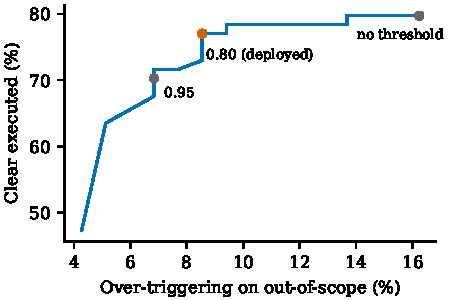
\includegraphics[width=\columnwidth]{figures/threshold.pdf}
\caption{Effect of the threshold for the deployed model on the clean test (descriptive; the threshold was chosen on the
calibration set).}
\label{fig:threshold}
\end{figure}

On the clean test the threshold consistently trades severe errors for mild ones. For the contrastive model ($\tau=0.90$,
chosen on validation) wrong actions fell from 53 to 33 and from 44 to 25 per seed (about $-40\%$); for LoRA v5 ($\tau=0.85$)
from 34/38 to 21/23; for the deployed model ($\tau=0.80$) from 41 to 29, with over-triggering on out-of-scope requests falling
from 16.2\% to 8.5\% (Figure~\ref{fig:threshold}). The price is extra confirmations: clear-command accuracy drops (e.g.\ LoRA v5
79.1 $\rightarrow$ 70.9), but every clear command lost this way was replaced by a confirmation proposing the correct call, so
the share solved after at most one ``yes'' is unchanged (59 = 52 + 7 items for seed 42). Thresholds must be re-chosen per
model: LoRA is less confident than full fine-tuning, 4-bit quantization lowers confidence further, and an under-trained model
lost every clear command at $\tau=0.90$.

Our first rule (largest $\tau$ that loses $\le1\%$ of clear commands on validation) was arbitrary, and validation contains too
few over-triggers to choose from (3--14). We therefore built a 194-sentence calibration set of hard out-of-scope requests and
asked for a guarantee: the lowest $\tau$ whose one-sided 90\% Clopper--Pearson bound \citep{clopper1934} on wrong behavior is
$\le10\%$. \emph{No model met it at any $\tau\le0.99$}: 19--28\% of these requests are handled wrongly without a threshold
and 9--16\% remain at $0.99$, because the model is confidently wrong. Separating the two kinds of error is informative:
self-executed wrong actions fall from 9--13\% to 3--5\% at $\tau=0.85$, and what the threshold cannot touch are
clarification proposals in response to chit-chat (``seeing these flame trees reminds me of school'' $\rightarrow$ ``open the
sunroof?''), a side effect of the story-like clarification data that is present in v5 and v6.1 alike. The deployed threshold
0.80 was chosen on this set (5 self-executed errors out of 194, as at 0.85, with fewer lost commands).

\subsection{Quantization and deployment}
\label{sec:quant}

The model is converted to GGUF and quantized with llama.cpp. The compression level was chosen by a rule fixed in advance on
validation and development data (3,036 items): accept the first of q4\_K\_M, q4\_K\_M+imatrix, q5\_K\_M, q8\_0 that loses at most
0.5\% of correct clear commands, adds at most two over-triggers and loses at most two ambiguous items relative to the unquantized
model. For v5, f16 conversion changed 5 of 3,036 outputs, q8\_0 5, q5\_K\_M 24 and q4\_K\_M 38; q4\_K\_M passed (q5\_K\_M failed by
one ambiguous item), so q4\_K\_M was chosen (Table~\ref{tab:quant}). llama.cpp keeps the output layer at 6 bits even in
q4\_K\_M, which protects the rows of the 27 new tokens. The f16 conversion on the same CPU reproduced the unquantized model, so
the remaining differences come from rounding, not from the hardware.

\begin{table}[t]
\centering\small
\setlength{\tabcolsep}{3pt}
\begin{tabular}{@{}lrrrrr@{}}
\toprule
v5, val+dev & Size & Clear & Over-trig. & Amb. & Same \\
\midrule
HF bf16 & 3.31\,GB & 1,506 & 14 & 127 & -- \\
f16 & 3.31\,GB & 1,508 & 14 & 126 & 3,031 \\
q8\_0 & 1.76\,GB & 1,507 & 15 & 126 & 3,031 \\
q5\_K\_M & 1.20\,GB & 1,505 & 13 & 124 & 3,012 \\
q4\_K\_M & 1.04\,GB & 1,503 & 12 & 125 & 2,998 \\
\bottomrule
\end{tabular}
\caption{Quantization of the v5 model on 3,036 validation and development items: correct clear commands, over-triggers,
correct ambiguous items and outputs identical to HF.}
\label{tab:quant}
\end{table}

\paragraph{Deployment on test.} After freezing everything, we scored the deployed v6.1 model once on all frozen sets. On
validation, q4\_K\_M had again passed the rule (+4 clear, +0 over-triggers, $-2$ ambiguous, 2,971 of 3,006 outputs identical),
yet on test it scored below the unquantized model run on GPU, most visibly on long implicit requests (Ambig-4 79.8
$\rightarrow$ 74.4) and short commands (88.3 $\rightarrow$ 82.5). To separate the effect of rounding from that of changing the
inference stack, we also converted the same model to f16 and q8\_0 GGUF and scored f16, q8\_0 and q4\_K\_M one after another on
the same CPU (Table~\ref{tab:deploy}; re-scoring q4\_K\_M reproduced all 701 earlier outputs). Two effects appear. First,
moving from batched bf16 inference on GPU to f16 on CPU already flips near-boundary items: on the small ambiguous group f16
scores 69.2 against 74.4. Second, relative to f16 on the same CPU, q4\_K\_M is significantly worse on short commands (0 vs.\ 7
flipped items, $p=0.016$) and close to significant on Ambig-4 (1 vs.\ 7, $p=0.070$), whereas q8\_0 gives the same output as
f16 for 680 of 701 prompts and differs significantly on no group. Validation items are confident (top-token probability near
0.99), so small numeric shifts rarely flip them; the human-reviewed sets contain many near-boundary decisions that do. We keep
q4\_K\_M because the choice was made by a fixed rule on non-test data, and note that this rule is not sensitive enough to
distribution shift. q8\_0 is the safer choice on stronger hardware: it is 1.7$\times$ larger and, in the same session, 1.8$\times$
slower than q4\_K\_M (median 856 vs.\ 463\,ms). With the threshold, all three levels make the same number of wrong actions on
the clean test (29). On the laptop CPU (i5-12500H, 8 threads) the deployed model needed 520\,ms at the median and 961\,ms at
the 95th percentile per decision in the first scoring session (463 and 832\,ms in the second).

\begin{table}[t]
\centering\small
\setlength{\tabcolsep}{2.5pt}
\resizebox{\columnwidth}{!}{%
\begin{tabular}{@{}lccccc@{}}
\toprule
v6.1 seed 42 & HF (GPU) & f16 & q8\_0 & q4 & q4 + 0.80 \\
\midrule
Clear (74) & 81.1 & 81.1 & 81.1 & 79.7 & 77.0 \\
Ambiguous (39) & 74.4 & 69.2 & 69.2 & 64.1 & 64.1 \\
Out-of-scope (117) & 82.9 & 82.1 & 82.1 & 82.9 & 88.0 \\
Ambig-4 (129) & 79.8 & 79.1 & 78.3 & 74.4 & 74.4 \\
Short + paraphr.\ (120) & 88.3 & 88.3 & 85.0 & 82.5 & 79.2 \\
Two-turn (60) & 66.7 & 66.7 & 65.0 & 61.7 & 56.7 \\
Typos (104) & 60.6 & 58.7 & 60.6 & 55.8 & 47.1 \\
Wrong actions, clean & 37 & 40 & 40 & 41 & 29 \\
Median latency (CPU) & -- & 1,062 & 856 & 463 & 463 \\
\bottomrule
\end{tabular}}
\caption{The deployed model (v6.1 seed 42) on the frozen test sets. HF: unquantized, batched bf16 on GPU. The other columns
are GGUF on the same laptop CPU in one session; latency in ms per decision (p95: 2,075 / 1,480 / 832). The threshold does not
change the model's own clarifications, so the ambiguous rows of the last two columns are identical.}
\label{tab:deploy}
\end{table}

\paragraph{Answer phrasing.}
\label{sec:turn2}
The model can also phrase the answer from the function result (second prompt). Measured with the v5 model on 200 validation
samples, it refused
correctly in 99 of 99 out-of-scope samples, and 87.1\% of informative answers passed the code checks (no invented number, no
English words), but it also produced semantic errors that no check caught (``today'' for a two-day forecast, a wrong pressure
comparison) and added a median 1.6\,s. The deployed system therefore answers with templates; model answers remain available
as an option.

\subsection{GRPO after distillation}
\label{sec:grpo}

Since the remaining errors are decisions (call, clarify or refuse), we tried GRPO \citep{shao2024deepseekmath} with a
code-computed reward that weights errors by their consequence: correct $+1$, unnecessary clarification $-0.2$, false refusal or
wrong proposal $-0.5$, unparseable $-1$, wrong action on the car $-5$. The magnitude $-5$ is tied to the runtime threshold:
acting at $p=0.8$ has the same expected reward as asking ($0.8\cdot1-0.2\cdot5=-0.2$). A fresh LoRA (r\,16) on the merged
v6.1 model was trained with TRL, $G=8$, learning rate $10^{-5}$, KL coefficient 0.04 and temperature 1.0 for two epochs on
about 4,000 training prompts on which v6.1 was uncertain ($p_{\text{top}}<0.95$, including lower-cased copies) plus 400
confident ones. A new 200-item test set (197 after removing 3 contaminated items, plus a lower-cased copy) was frozen before
training, together with five acceptance criteria.

\begin{table}[t]
\centering\small
\begin{tabular}{@{}lccc@{}}
\toprule
Criterion (mean of 2 seeds) & v6.1 & GRPO & \\
\midrule
(1) Wrong actions $\downarrow$ & \textbf{6.3\%} & 6.9\% & fail \\
(2) Implicit (M) & 80.1 & 81.2 & pass \\
(3) Clear (R) & 85.0 & 85.0 & pass \\
(4) False refusals $\downarrow$ & 1.3\% & \textbf{0.6\%} & pass \\
(5) Unneeded clarif.\ in R & 0.0 & 0.0 & pass \\
\bottomrule
\end{tabular}
\caption{GRPO vs.\ its starting point on the GRPO test set (original and lower-cased copies). GRPO had to reduce wrong actions
without hurting the other criteria.}
\label{tab:grpo}
\end{table}

GRPO failed the main criterion (Table~\ref{tab:grpo}). It barely changed the model: at the end of training 81--87\% of the
8-sample groups had identical rewards (no learning signal), the largest weight change in a query projection was
$2.4\times10^{-4}$, and only 1--16 of 197 items changed outcome per evaluation. Seven items flipped from correct to a wrong
action (unsupported features close to real ones, such as ``honk the horn'' or ``lane-departure warning'') and three in the
other direction, a difference within noise. GRPO did improve what it practiced: 60\% of the uncertain prompts were lower-cased
copies, and false refusals on lower-cased input fell from 8 to 3 for one seed---a problem the runtime already solves by
capitalization. Compared with tool-use RL that succeeds \citep{qian2025toolrl,zhang2025tooln1}, our setting lacks a reasoning
step (the decision is one token, so sampling explores little), and our prompts were already solved by the model, whereas DAPO
\citep{yu2025dapo} continuously filters such groups. We keep v6.1 and report GRPO as a negative result (cost about US\$2.2).
